\problemname{Race Track}

Racing is a lot of fun, but it's only fun when you are driving at 300 kph on the track; when you are off track, you can only drive very slowly and that's not fun for anyone.

Anthony likes to go racing, but he faces a difficult problem. When Anthony tries to enter the race track, a helicopter would pick him up in his car, fly him to the track, and drop him off. However, the helicopter pilot isn't always very good; he would sometimes drop Anthony at a point that's not on the track. When this happens, Anthony has to drive back on track so he can finally have some fun. Since driving off track is unbearably boring, Anthony wants to minimize the amount of distance driving off track.

Anthony enters and leaves the race track multiple times during one race session, and every time the pilot drops him off, he would like to know the shortest distance he can travel to get back on track.

A track is defined as a polygon (not necessarily simple) whose corners may or may not be smoothed. A corner is said to be smoothed by length $L$ when each of the edges connected to the corner is sliced by length $L$, and are then reconnected by an arc, such that the resulting curve is smooth, i.e. at least $C^1$ continuous.

\begin{figure}[h]
\begin{center}
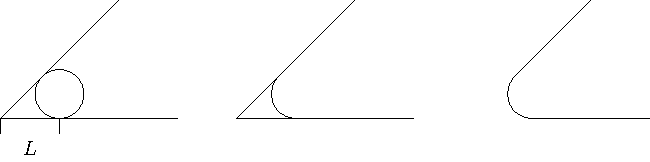
\includegraphics{picture1.pdf}
\caption{A corner of 45 degrees smoothed by length $L$.}
\end{center}
\end{figure}

Figure \ref{fig:track} shows a polygon; coincidentally it's a square with length 2. The polygon then has its top right corner smoothed by 1.

\begin{figure}[h]
\begin{center}
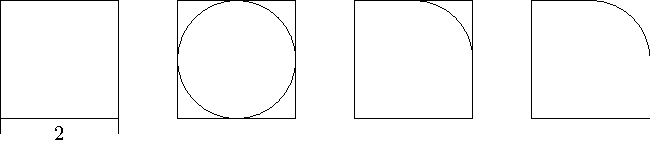
\includegraphics{picture2.pdf}
\caption{A track with 1 smoothed corner.}
\end{center}
\label{fig:track}
\end{figure}

Write a program to help Anthony figure out the shortest distance he can travel to get back on track!

\section*{Input}

The first line of input contains two integers $3 \leq N \leq 10^6$, the number of points of the polygon, and $1\leq Q\leq 100$, the number of queries, i.e. the number of times Anthony enters the track with a helicopter.

$N$ lines follow, the $i$-th line contain 2 real numbers, $-10^6\leq X_i,Y_i\leq 10^6$, the position of $P_i$, the $i$-th point.

$N$ more lines follow, the $i$-th line contain a single real number, $0\leq L_i\leq 10^6$, the smoothing length for the corner $P_{i}$.

It is guaranteed that for all $i$, $L_i+L_{i+1}$ is at most the length of the line formed by $P_i$ and $P_{i+1}$.

It is also guaranteed that all interior polygon angles are either at most 175 or at least 185.

$Q$ lines follow, each line contains 2 real numbers, $-10^6\leq X,Y\leq 10^6$, where the pilot drops off Anthony. This indicates a query. It is \emph{not} guaranteed that position $(X,Y)$ is off the track; sometimes the pilot actually flies decently.

\section*{Output}

For each query, output a single line containing a real numbers, the closest distance between point $(X,Y)$ and a point on the track.
Your answer will be considered correct if its absolute or relative error doesn't exceed $10^{-5}$.

